\section*{Источники и решения}

\subsubsection*{Торт-мороженое}

Эта замечательная головоломка досталась мне от французского аспиранта Тьерри Мора,
а тот узнал её от своего школьного учителя Томаса Лаффорга.
Головоломка (происхождения которой Лаффорг точно не знает) на самом деле включала в себя ещё один угол, определяющий зазор между дольками торта.
Даже в этом случае, глазурь ухитрится вернуться наверх после конечного числа операций;
упорные читатели могут в этом убедиться.
Наша формулировка (с нулевым зазором) уже достаточно удивительна и, думается, достаточно сложна.

Если вы решили, что при иррациональном $x$ понадобится бесконечное число операций, то вы совсем не одиноки.
В конце концов, если $n$ операций достаточно, то $n$-й разрез, должен пройти по границе области покрытой глазурью;
как же смогла эта линия оказаться там, где торт никогда не разрезался?

Однако она там окажется.
Причина в том, что когда долька переворачивается, её покрытая и непокрытая области  меняются не только местами, но и порядком.

В этой головоломке, как и во многих алгоритмических задачах, полезно переопределить операцию так, чтобы менялось только состояние (в данном случае, область, покрытая глазурью), а не сама операция, которая пока что у нас меняется на каждом шагу.
В нашем случае достаточно добавить поворот торта после каждой операции так, чтобы разрез всегда приходился на одно и то же место.


\begin{figure}[htb!]
\centering
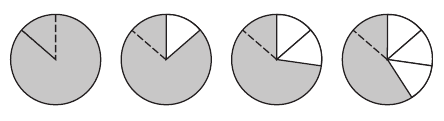
\includegraphics[scale=.9]{pics/tort2}
\caption{Разрезы и перевороты с вращением.}
\label{pic:tort2}
\end{figure}

Будем считать, что $0\degree$ --- направление на север,
$90\degree$ --- на восток и так далее.
Каждый раз будем разрезать по направлениям $0\degree$ и $-x$.
Затем кусок переворачивается через линию $0\degree$ и оказывается между $0\degree$ и $x$.
В это же время остальная часть торта поворачивается по часовой стрелке на угол~$x$.
На рис. \ref{pic:tort2} пунктирные линии показывают где проходят разрезы на первых четырёх шагах.

Чтобы понять дальнейшее рассуждение, проще всего думать, что $x$ чуть больше $360\degree/k$ для некоторого целого $k$.
В этом случае первый разрез по уже отрезанной дольке произойдёт на $k$-м шаге, после того как торт развернётся на полный оборот.

И так, пусть $k$ --- наименьшее число долек, которое надо вырезать, чтобы добраться до конца торта.
Другими словами, $k$ --- наименьшее целое число, большее или равное $360\degree/x$.
Тогда $x \z= y + z$, где $y = 360\degree/k$ и 
\[0\le z <\frac{360\degree}{k-1}-\frac{360\degree}{k}=\frac{360\degree}{(k-1)k}.\]
Конечно же, если $z = 0$, то $x = y = 360\degree/k$, и тогда $k$ операций переведут всю глазурь на дно торта, а ещё $k$ вернут её наверх.
В противном случае, как мы увидим, невозможно достичь момента, когда вся глазурь окажется снизу.

По мере выполнения шагов будут появляться граничные линии (между покрытой и непокрытой областями) под углами $0$, $x$, $2x$, $3x, \z\dots , (k - 1)x$, а затем $x - kz$, $2x - kz$, $3x - kz, \dots , (k - 1)x - kz$,
и затем они повторяются.
Действительно, легко проверить, что описанный набор граничных линий, скажем, $S$, замкнут относительно операции разрез-переворот-поворот.
Одна такая операция переносит $ix$ в $(i + 1)x$, кроме $(k - 1)x$, который переносится в $x - kz$;
она же переносит $ix - kz$ в $(i + 1)x - kz$, кроме $(k - 1)x - kz$, который идёт в $x$.
Тем временем разрез $0\degree$ всё время остаётся на месте.
Отсюда следует, что набор граничных линий всегда является подмножеством $S$.

Уже можно заключить, что конечное число операций вернёт всю глазурь на верх, ведь у нас только $2k - 1$ областей торта между $2k - 1$ линиями из $S$.
Каждая область может быть покрыта или не покрыта глазурью, поэтому число достижимых конфигураций не превышает $2^{2k-1}$.
Значит, процесс зациклится не позднее чем за $2^{2k-1}$ шагов.
Но обязательно ли мы вернёмся к начальной конфигурации (все области покрыты глазурью)?
Да, потому что операция обратима.
Если бы процесс зациклился на другой конфигурации $C$, то существовали бы две разные конфигурации, которые приводили бы к $C$, а это невозможно.

\begin{figure}[hbt!]
\centering
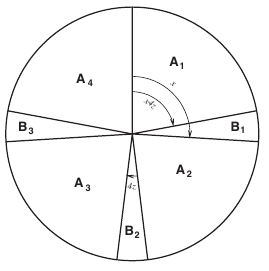
\includegraphics[scale=1]{pics/tort3}
\caption{Области при $x = 93{,}5\degree$ и значит $z = 3{,}5\degree$.}
\label{pic:tort3}
\end{figure}

Однако несложно понять в точности, что и как происходит.
Между граничными линиями в $S$ есть $k$ областей с углом $x - kz$ --- назовём их $A_1$, $A_2, \dots , A_k$, и ещё $k - 1$ область с углом $kz$ --- назовём их $B_1$, $B_2, \dots , B_{k-1}$.
(На рис. \ref{pic:tort3} показан случай $k = 4$ при $x = 93{,}5\degree$.)

С начала процесса, $A$-области становятся не покрытыми глазурью, по порядку.
После $k$ операций они все без глазури.
Затем они снова покрываются глазурью, снова по порядку, до тех пор, пока после $2k$ операций все покроются глазурью.
Тем временем $B$-области также становятся не покрытыми по порядку.
Поскольку их только $k - 1$, после $k - 1$ шагов все они станут не покрытыми, и все снова покроются после $2k - 2$ шагов.

Значит число шагов, необходимых чтобы покрыть глазурью оба типа областей, равно наименьшему общему кратному $2k$ и $2k \z- 2$, то есть $2k(k - 1)$.
Значит потребуется $2k(k - 1)$ шагов, конечно если $x \z\ne 360\degree/k$ ---
в этом случае $B$-области отсутствуют и достаточно $2k$ шагов.

Рассуждая таким же образом, заключаем, что если все области не покрыты глазурью после $n$ шагов,
то $n$ равно нечётному числу домноженному на $k$
и в то же время нечётному числу домноженному на $k - 1$.
Поскольку ровно одно из чисел $k$ и $k - 1$ нечётно, $n$ чётно и нечётно одновременно,
что невозможно.
Значит, если есть $B$-области, то вся глазурь никогда не окажется снизу.

А вот реакция на эту головоломку одного очень известного математика:
«Трудно поверить, что вся глазурь вернётся наверх.
Но если уж это произойдёт, то я уверен, что в какой-то момент вся глазурь окажется снизу!»

\begin{addedbytheeditors}
\textbf{Редакторам:} 
На рис. \ref{pic:tort2} надо добавить отметить отрезок штрихованной линией на первом кружке.
На рис. \ref{pic:tort3} надо поменять $x4z\to x-4z$.
\end{addedbytheeditors}

\subsubsection*{Прыгание и перепрыгивание}

Эту, на вид, простую головоломку придумал Джеймс Б. Ширер --- математик из IBM.
Она появилась на сайте головоломок IBM \cite[апрель 2007]{ponder-this}.
Головоломка вовсе не такая простая, хоть и колется парой полезных приёмов.

Пронумеруем кувшинки по порядку.
Естественно начать с подсчёта вероятности $p$ того, что лягушка, стартуя с $1$, вернётся в какой-то момент в $0$.
Чтобы никогда не возвращаться, ей придётся совершить прыжок вперёд (вероятность $1/2$) и не вернуться обратно трижды (вероятность $1 - p^3$).
Таким образом, $(1 - p) = \tfrac12(1 - p^3)$.
Поделив на $(1 - p)/2$, получим, что $2 = 1 + p + p^2$, а это даёт $p = (\sqrt5 - 1)/2 \z\sim 0{,}618034$ --- знакомое золотое сечение.

Однако подсчитать вероятность того, что лягушка перескакивает конкретную позицию (скажем, $1$), так легко не получается.
Можно было бы начать вычисления с момента, когда лягушка первый раз попадёт в $0$; ведь если это не произошло, то ей придётся попасть в~$1$.
Однако легче вычислить вероятность того, что во время конкретного прыжка лягушка перескакивает через кувшинку, которую она  не посещала и не посетит.

Для того чтобы это произошло, лягушка должна
(а) прыгать вперёд в данный момент,
(б) никогда не возвращаться обратно от того места, где она приземлилась,
и (в) не посещать ту кувшинку, через которую она прыгает, в прошлом.

Можно считать, что кувшинка, которую перепрыгивает лягушка, стоит под номером 0.
Ключ в том, что если развернуть нумерацию и время, то событие (в) становится независимой копией события (б).
Иначе говоря, лягушка ведёт себя ровно так же, если обратить время и рассматривать кувшинки в обратном порядке ---
она равновероятно прыгает на два вперёд или на один назад.
Событие (в) означает, что «достигнув» $-1$, она не «вернётся» в $0$.

Таким образом, вероятность того, что все три события произойдут, составляет $1/2 \cdot (1 - p) \cdot (1 - p) = (1 - p)^2 / 2$.
Однако это ещё не вероятность того, что $0$ пропускается, а только вероятность того, что в данный момент лягушка перепрыгивает через пропущенную кувшинку.

Поскольку лягушка, в среднем, перемещается со скоростью $1/2$, она производит $(1 - p)^2$ пропущенных кувшинок на единицу пройденного пути.
Отсюда следует, что доля кувшинок, на которые она попадает, составляет $1 - (1 - p)^2 \z= (3\sqrt5 - 5) / 2 \sim 0{,}854102$.

\subsubsection*{Три тени кривой}

Эту головоломку мне подбросил Рик Кенион (Университет Британской Колумбии), который увидел её на двери Джорджа Бергмана в Бёркли. 
Бергман услышал её от Хендрика Ленстры из Бёркли и Университета Лейдена.
По словам Бергмана, Ленстра видел игрушку, состоящую из кубической пластиковой коробки с прорезями, образующими своего рода лабиринт на каждой грани.
При этом каждая пара противоположных граней имела одинаковые прорези, так что стержень, перпендикулярный этим двум граням, мог двигаться, проходя через эти два лабиринта.
Но вместо одного стержня был объект, который, по сути, состоял из трёх взаимно перпендикулярных стержней, соединённых в точке, и каждый стержень проходил через лабиринты на паре противоположных граней коробки.
Требовалось добраться из одной позиции в другую.

\begin{figure}[b!]
\centering
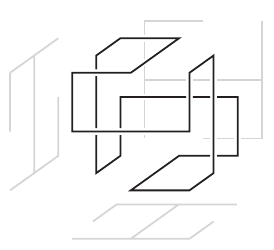
\includegraphics[scale=1]{pics/tree3}
\caption{Кривая три тени которой деревья.}
\label{pic:tree3}
\end{figure}

Кстати, эту головоломку теперь можно приобрести.
%ссылка не работает??? http://bitsandpieces.com/ˆBrainteasersˆMetal+Puzzles/07-W7871.html. 
Её придумал Оскар ван Девентер --- блестящий голландский изобретатель, чьи механические головоломки часто воплощают увлекательные математические идеи.

Так или иначе, Ленстра обратил внимание на то, что лабиринт на каждой грани коробки обязан быть деревом;
если бы он имел замкнутый цикл, то вывалилась бы часть пластика.
Тогда он задался вопросом, какова будет область доступных позиций для центральной точки трёх стержней.
Её проекция на каждую грань должна быть деревом, но может ли это множество само иметь цикл?
Если да, то такой цикл должен был проецироваться на каждую грань как дерево.
Так и возник вопрос.

Ленстра задумался над этим в феврале 1994 года, или около того.
Бергман расспрашивал об этом разных людей, но безуспешно.
Наконец, в сентябре 1995 года Кевин Базард, в то время постдок в Бёркли, сообщил Бергману и Ленстре, что вопрос был известен ещё раньше в Кембридже (Англия), и нашёлся пример.
Базарду этот пример показал Имре Лидер, комбинаторик из Кембриджского университета, который услышал о нём от Джона Рикарда, который его и придумал.
Тогда Рикард работал на математическом отделении Кембриджа, но теперь программист.

Пример Рикарда, который обладает очень красивой шестикратной симметрией, изображён на рис. \ref{pic:tree3}.

\subsubsection*{Игроки и победители}

Эта задача пришла ко мне от Алона Орлицкого из Университета Калифорнии в Сан-Диего.
Она иллюстрирует силу коммуникации \emph{от студента к учителю}.

Тристан и Изольда могут заранее пометить команды четырёхзначными двоичными кодами от 0000 до 1111 в алфавитном порядке.
Затем, когда Тристан узнает, кто играл, он может отправить Изольде 00, 01, 10 или 11 передав \emph{первую позицию в которой отличаются две метки команды} --- это может быть первый, второй, третий или четвёртый бит.
Изольде следует отправить обратно значение этого бита.

Например, если команда 0110 играла с командой 0011 и одержала победу,
то Тристан отправит Изольде «01», указывая, что метки играющих команд отличаются во втором бите.
Изольда отправит обратно «1» --- значение второго бита победившей команды.

Эта схема требует отправки трёх битов --- на один меньше, чем метод, при котором Изольда просто отправляет метку победившей команды.
Однако на самом деле этот бит обеспечивает экспоненциальное улучшение!
Если у нас $n = 2^{2^k}$ команд, то один метод требует $2^k$ битов, а другой всего $k + 1$.


\begin{addedbytheeditors}
 \textbf{Редакторам:} Возможно «от студента к учителю» надо переводить иначе.
Кто-нибудь владеет терминологией сложности коммуникаций?
 \end{addedbytheeditors}

\subsubsection*{Подсказка для Чарли}

На самом деле это серьёзная задача по сложности коммуникаций.
Она была рассмотрена Лесом Валиантом из Гарварда в 70-х годах,
а сообщил мне о ней Амит Чакрабарти из Дартмутского колледжа.
Решения этой и более общей задачи приведены в статье Павла Пудлака, Войтеха Рёдля и Йижи Шгалла \cite{49}.

Пусть $x_1, \dots , x_n$ --- биты, представляющие ответы, где (допустим) $1 = \text{«да»}$ и $0 = \text{«нет»}$.
Индексы берутся по модулю $n$.
Алиса отправляет Чарли $x_{-i}$,
а Боб отправляет Чарли все значения $x_a + x_b$ для всех пар $(a, b)$, таких что $a + b = j$ и $a\ne b$;
сумма битов берётся по модулю $2$.
Обратите внимание, что таких пар не больше чем $n/2$.

Чарли знает $x_{-i}$, а также $x_{-i} + x_{i+j}$, сложив их, он получит $x_{i+j}$.

Выглядит просто, но догадаться сложно.

\begin{addedbytheeditors}
\textbf{Редакторам:} Добавил $a\ne b$ и заменил не совсем верную фразу:
``Notice that there are n/2 such pairs (after rounding up
when n is odd).''
\end{addedbytheeditors}

\subsubsection*{Сближение по кривой}

Этим вопросом меня озадачил Оскар ван Девентер, тот, что уже упоминался выше.
Он думал использовать такую кривую в механической головоломке.
Такие кривые на самом деле существуют, сложнее найти пример для которого несложно доказать, что он не обладает вторым свойством.

На рис. \ref{pic:ss-curve} показана такая кривая, которую по своим причинам ван Девентер называет \emph{неконкинкульной}.
%non-conquinculous

\begin{figure}[htb!]
\centering
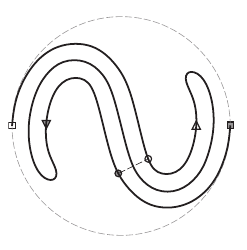
\includegraphics[scale=1]{pics/ss-curve}
\caption{Кривая со свойством (1), но без сойства (2).}
\label{pic:ss-curve}
\end{figure}

Пунктирная окружность на рисунке добавлена для того, чтобы было ясно, что кривая удовлетворяет первому свойству.
Остаётся убедиться, что для неё второе свойство не выполнено.
Предположим обратное, и пусть $t$ --- первый момент времени, когда один карандаш пройдёт от белого квадрата до белой стрелки,
либо же другой --- от серого квадрата до серой стрелки.
Какое-то время \emph{до} момента $t$ два карандаша окажутся друг напротив друга, как белый и серый круги.
Но \emph{после} времени $t$ им придётся разойтись, чтобы сойтись вместе, и это приведёт к увеличению расстояния.

Но как же догадаться до такой кривой?
(Если вопрос пугает, то пропустите следующие три абзаца.)
Представьте себе, что кривая параметризована параметром $t$;
это означает, что существует непрерывная функция $C$ из $[0, 1]$ в плоскость такая, что $C(0)$ --- один конец кривой (скажем, левый), $C(1)$ --- другой её конец, и $C(t)$ описывает кривую когда $t$ бежит от $0$ до $1$.
Успешное управление карандашами в соответствии со свойством (2) подразумевает пару непрерывных функций $f$ и $g$ из $[0,1]$ в себя, где в момент времени $t$ карандаши расположены в точках $C(f(t))$ и $C(g(t))$.
Таким образом, $f (0) = 0$, $g(0) = 1$, $f (1) = g(1)$, и расстояние от $C(f (t))$ до $C(g(t))$ не возрастает по $t$.
Вместе $f$ и $g$ описывают кривую от точки $(0,1)$ до линии $x = y$, в треугольнике с вершинами в $(0,1)$, $(0,0)$ и $(1,1)$.

Для того чтобы это стало невозможным, хотелось бы иметь \emph{двойственный путь} между прямыми $x = 0$ и $y = 1$, не выходящий на $x = y$, и соответствующий парам точек на локально минимальном расстоянии.
Такая кривая обязана пересечься с нашей кривой $(f, g)$, а это влечёт подъём расстояния.

Этот двойственный путь соответствует другому виду манипуляций с карандашами:
начинаем с левого карандаша в левой конечной точке и правого карандаша где-то на кривой,
затем перемещаем обе точки в одном направлении вдоль кривой, пока правый карандаш не достигнет правой конечной точки.
Если при этом ни одну точку нельзя переместить относительно другой без увеличения расстояния между ними, то мы достигли цели.
На данной фигуре карандаши начинают с белого квадрата и серой стрелки, затем движутся вместе, пока не достигнут белой стрелки и серого квадрата, соответственно.

\medskip

В награду за этот пример ваш автор получил прототип механической головоломки, замечательной как и все творения ван Девентера.

\subsubsection*{Суммы и произведения}

Эта забавная головоломка всплывала на различных формах в течение многих лет; она появилась в колонке Мартина Гарднера для Scientific American в декабре 1979 года, но по какой-то причине не вошла в сборник задач этой колонки \cite{29}.
Кажется удивительным, что столь туманной информации может хватить.

Головоломка (по сути, та же, что наша) была предложена независимо Стивом Феннером из Университета Южной Каролины и Биллом Готтесманом, разработчиком и производителем солнечных часов.
Ход рассуждений ниже предложен Готтесманом.

Для начала обозначим число Порфирио через $P$, а число Саманты через $S$, и пусть $\{X, Y\}$
--- неизвестная пара.
Вначале Порфирио не знает ответа, значит числа $X$ и $Y$ не могут быть оба простыми,
ни простым и его квадратом,
ни простым и его кубом.
Более того, ни одно из них не может быть большим простым числом (больше чем $50$), так как в этом случае оно должно было бы быть одним из сомножителей~$P$.

Следовательно, поскольку Саманта заранее знает, что Порфирио не может знать ответ,
$S$ не может превзойти $53$ или же быть равным сумме двух простых чисел.
Это исключает все чётные числа --- гипотеза Гольдбаха, проверенная далеко за $53$, гласит, что каждое чётное число больше $2$ представимо как сумма двух простых.
Остаются только некоторые из чисел, превышающие какое-то нечётное составное число на $2$, а именно
$11$, $17$, $23$, $27$, $29$, $35$, $37$, $41$, $47$ и $53$.
Готтесман назвал эти числа \emph{золотыми}.
(Например, $51=34+17$ и число $34\times 17$ допускает единственное разложение на сомножители до $100$.
Поэтому $51$ не золотое, хотя и превышает на $2$ составное число $49$.)
Не нужно беспокоиться о суммах простого числа и его квадрата или куба, так как они все чётные.

Из того, что Порфирио теперь уже знает $X$ и $Y$ (и из того, что сумма и произведение двух положительных целых чисел полностью их определяет), выводится, что множители всего одного разложения $P$ дают золотую сумму. 
Каждое золотое число $G$ даёт Саманте $(G - 3)/2$ возможных пар $\{X, Y\}$
(например, для $11$ можно собрать как $2 + 9$, $3 + 8$, $4 + 7$ или $5 + 6$); должно оказаться, что только одна из этих пар имеет произведение $P$ с желаемым свойством.

Если $G = 11$, то первые две пары выше уже позволяют Порфирио найти $X$ и $Y$.
Для случая $2 + 9$, получаем $P = 18$, и оно раскладывается только как $2 \times 9$ (где $2 + 9 = 11$ является золотым) или как $3 \times 6$ (дающее не золотую сумму $S = 9$).
В случае $3 + 8$ получаем $P = 24$, оно раскладывается как $2 \times 12$ (а $14=2+12$ не золотое) или
$3 \times 8$ (и $11=3+8$ золотое) или $4 \times 6$ (а $10=4+6$ не золотое).
Таким образом, $G$ не может быть $11$.

Следующее золотое число, $17$, подходит!
Ровно одна пара слагаемых даёт $P$, у которого единственная золотая сумма множителей равна $17$, а именно $4$ и $13$ (поскольку $2 + 26 = 28$, не золотое).

Надо ещё перебрать остальные шесть пар слагаемых для $17$, чтобы убедиться, что ни одна из них не даёт подходящего $P$.
Это даёт надежду, что $X$ и $Y$ могут быть $4$ и $13$.
Остаётся проверить, что $\{4, 13\}$ --- единственный ответ.
Для этого придётся повторить весь процесс для остальных восьми золотых чисел, 
и мы убедимся, что ни одно из них не подходит.

Решение этой головоломки не достаточно изящно,
хоть я и объявил это необходимым требованием (для решённых головоломок).
Однако то, что услышав этот короткий разговор, можно восстановить числа, не зная ни суммы, ни произведения, служит небольшим вознаграждением.

\begin{addedbytheeditors}
\textbf{Редакторам:}
Я не понял зачем говорить о квадратах и кубах.
И не понял почему не золотые 23 и 29.
(И нет охоты понимать.)
Почему там стоит 53? --- 53 это первое простое после 50, а числа начинаются с 2 --- вроде должно быть 54?
(Последнее конечно не влияет на рассуждение.) 

Кто-то должен это переписать.
\end{addedbytheeditors}

\subsubsection*{Сложенный многоугольник}

Эта головоломка пришла ко мне (как открытый вопрос) от Роберта Вейта из Юго-Восточного университета Индианы, который долго и тщетно пытался её решить.
Мне удалось найти (на мой взгляд) изящное решение, представленное ниже.
Позже выяснилось, что задачу уже решили К. Бёроцки, Г. Кертеша и Э. Макая \cite{9}.

Ответ такой: у каждого нечётноугольника с единчными сторонами площадь не меньше $\sqrt{3}/4$, причём равенство достигается только для треугольника.

Как такое доказывается?
Утверждение тривиально для треугольников,
и естественно возникает искушение воспользоваться индукцией по числу сторон.
Как мы увидим,  многоугольник с четырьмя и более сторонами разрезается диагональю на два многоугольника с меньшим числом сторон у каждого.
Однако, вообще говоря, новые многоугольники не будут равносторонними.
Таким образом, нужно придумать индукционное предположение применимое к более широкому классу многоугольников, возможно, ко \emph{всем}.

Приведённое ниже индукционное предположение отлично работает, хоть и выглядит топорно.
Важно правильно подобрать параметр.

Обозначим через $\mathbb{O}^n$ множество всех целочисленных $n$-векторов нечётного веса, то есть 
\[\mathbb{O}^n=\left\{\,\vec x=(x_1,\dots,x_n)\in \mathbb{Z}^n\,\middle|\, \sum_ix_i\equiv 1\pmod 2\,\right\}.\]
Чтобы измерить, насколько многоугольник $P$ близок к нечётноугольнику с единичными сторонами, мы воспользуемся параметром $u(P)$, назовём его \emph{нескладностью} $P$, определённым как
\[u(P)=1-\min_{\vec x\in \mathbb{O}^n} \left\{\sum_i |e_i-x_i|\right\}.\]
где  $e_1,\dots,e_n$ --- длины сторон $P$.
Заметим, что $u(P)\z\leqslant1$, и $u(P)\z=1$ если $P$ --- нечётноугольник с единичными сторонами или даже любой многоугольник с целочисленными сторонами и нечётным периметром.
С другой стороны, $u(P)\leqslant 0$ если, например, две из сторон многоугольника $P$ имеют длину $\tfrac12$, или же если у него чётный целый периметр.

Многоугольник будет считаться \emph{хорошим}, если у него нет вырожденных вершин,
то бишь нет вершин с внутренним углом $180\degree$.
Если $P$ имеет стороны длины больше~$1$, то из него можно получить (возможно нехороший) многоугольник $P^*$ со сторонами длины не более~$1$, подразбив каждую длинную сторону $P$.
При этом, можно добиться что бы $u(P^*)=u(P)$.

Теперь мы переходим к индукционному доказательству того, что площадь $A(P)$ любого многоугольника $P$ не меньше $\tfrac{\sqrt{3}}{4}u(P)$.
Отсюда немедленно последует, что площадь нечётноугольника с единичными сторонами не меньше  $\sqrt{3}/4$.

Ключ к доказательству --- \emph{субаддитивность} функции $u(P)$;
то бишь $u(P)\leqslant u(Q)+u(R)$, где $P$ --- многоугольник (возможно нехороший) и диагональ, скажем $D$, делит его на многоугольники $Q$ и~$R$.

Докажем субаддитивность.
Пусть  $e_1,\dots,e_n$ --- длины сторон $P$, а его диагональ $D$ имеет длину $d$. 
Выберем $\vec x\in\mathbb{O}^n$ такой, что $u(P)\z=1-\sum_i |e_i-x_i|$.

Пусть $I$ --- множество индексов сторон $P$, которые также являются сторонами $Q$, а $J$ --- индексы сторон $R$.
Обозначим через $\vec x|I$ и $\vec x|J$ сужение $\vec x$ на стороны (кроме диагонали) $Q$ и $R$ соответственно;
можно предположить, что $\vec x|I$ имеет нечётный вес.
Пусть $d_0$ --- ближайшее к $d$ чётное целое число, а $d_1$ --- ближайшее к $d$ нечётное целое число, так что $|d_1-d_0|=1$.

Взяв $\vec x|I$ вместе с $D$-координатой $d_0$ для $Q$ и 
$\vec x|J$ вместе с $D$-координатой $d_1$ для $R$, получим
\begin{align*}
u(R)+u(Q)
&\geqslant
1-\sum_{i\in I}|e_i-x_i|-|d_0-d|
+
1-\sum_{i\in J}|e_i-x_i|-|d_1-d|
=
\\
&=
2-\sum_{i}|e_i-x_i|-1=
\\
&=u(P),
\end{align*}
что и требовалось.

Теперь докажем главное утверждение для \emph{маленьких} треугольников.
А именно, если $T$ --- треугольник со сторонами не длинней $1$, то 
$A(T)\geqslant \tfrac{\sqrt{3}}{4}u(T)$.
Более того, равенство достигается только для равностороннего треугольника с единичными сторонами.

Пусть длины сторон треугольника равны $a$, $b$ и $c$.
Можно предположить, что целочисленный вектор, дающий $u(T)$, либо $(1, 0, 0)$, либо $(1, 1, 1)$.
Поскольку $a < b + c$, в первом случае имеем $u(T)\z=1-(1-a)-b-c<0$, и значит нечего доказывать.

Во втором случае
$u(T)=1-(1-a)-(1-b)-(1-c)=2s-2$, где $s=\tfrac12(a+b+c)$ --- полупериметр треугольника.
Можно считать, что $s > 1$, иначе опять нечего доказывать.
В частности, каждое из чисел $a+b$, $b+c$ и $c+a$ больше $1$.

Мы утверждаем, что при данном $s$, треугольник $T$ имеет наименьшую площадь если две из его сторон единичные (а третья, соответственно, длины $2s - 2$).

Дабы это увидеть, зафиксируем $a$. 
По формуле Герона (её красивое доказательство можно найти в \cite{39}) получаем
\[\frac{A(T)^2}{s(s-a)}=(s-b)(s-c)=s^2-(b+c)s+bc.\]
Поскольку сумма $b + c$ постоянна, минимум достигается, если $b = 1$ или $c = 1$.

Далее, переобозначив стороны, можно считать что $a = 1$.
Повторив рассуждение, получим уже две единичные стороны.
Иначе говоря, площадь $T$ не меньше площади треугольника со сторонами $1$, $1$, $2s - 2$, то есть \[\sqrt{s(s-1)(s-1)(2-s)}.\]

Поскольку $s\in(1,\tfrac32]$, получаем, что $s(2-s)\geqslant \tfrac34$.
Значит 
\[A(T)\ge \sqrt{\tfrac34(s-1)^2}=\tfrac{\sqrt{3}}2(s-1)=\tfrac{\sqrt{3}}4u(T),\]
и равенство достигается только при $s=\tfrac32$.

Перейдём к доказательству основного утверждения.
Предположим, оно неверно.
Тогда найдётся хороший многоугольник $P$ с минимальным числом сторон, скажем $n$, такой, что $A(P)<\tfrac{\sqrt{3}}4 u(P)$.
Если $n=3$, упорядочим треугольники лексикографически по ($\lceil c\rceil$, $\lceil b\rceil$, $\lceil a\rceil$), где 
$a\leqslant b\leqslant c$ --- длины сторон $P$, и потребуем, чтоб $P$ был минимальным в этом (частичном) порядке.

Предположим сначала, что $n>3$, и пусть $D$ --- любая внутренняя диагональ~$P$.
Такая диагональ найдётся, потому что если $P$ выпуклый, то любые две не соседние вершины соединяются отрезком внутри $P$.
В противном же случае есть вершина $v$ с внутренним углом больше $180\degree$.
Если отсканировать внутренность $P$ из $v$, начиная с направления одной из сторон при $v$ и заканчивая другой,
то мы увидим более чем одну из оставшихся сторон.
Там, где сканирование переходит от одной такой стороны к другой, мы увидим вершину, с которой и можно соединить $v$ диагональю.

Можно считать, что диагональ разбивает $P$ на хорошие многоугольники $Q$ и $R$, каждый с менее чем $n$ сторонами и, следовательно, каждый удовлетворяющий неравенству теоремы.
Но по субаддитивности, 
\[A(P)<u(P)\leqslant \tfrac{\sqrt{3}}4(u(Q)+u(R))\leqslant A(Q)+A(R)=A(P)\]
--- противоречие.

Остаётся рассмотреть случай $n=3$.
Пусть $A$ --- вершина противоположная стороне $a$, и так далее.
Из рассмотрения маленького треугольника, мы знаем что $\lceil c\rceil>1$.
Если $\lceil b\rceil<\lceil c\rceil$, проведём диагональ от $C$ к любой новой вершине $P^*$;
длина этой диагонали меньше, чем $b$, так как углы, прилегающие к длинной стороне, острые.
Оба треугольника, на которые эта диагональ разбивает $P^*$, лежат ниже $P$ в лексикографическом порядке.
Применив субаддитивность, приходим к противоречию.

В случае если $\lceil c\rceil=\lceil b\rceil>1$, выберем $P^*$ так, чтобы на стороне $b$ (соответственно на стороне $c$) на расстоянии $1$ от вершины $C$ (соответственно от вершины $B$) была новая вершина $U$ (соответственно $V$).
Проведём две диагонали, одну от $U$ к $V$% (длиной $d$)
, и другую от $V$ к $C$% (длиной $e$)
.
Снова, применив субаддитивность, заключаем, что один из трёх полученных треугольников $BCV$, $CVU$ и $VUA$, должен быть контрпримером.
Однако все эти треугольники предшествуют $P$ в лексикографическом порядке, и это противоречие завершает доказательство.

Остаётся заметить, что индукция, вместе со строгим неравенством для маленьких треугольников, влечёт строгость неравенства для любого хорошего многоугольника $P$, если только $P$ сам не равносторонний треугольник с единичными сторонами.

Уф!
